\documentclass[a4paper,12pt,fleqn,bibliography=totoc,twoside]{scrreprt}
%fleqn 			--- macht die formeln links stat mittig
%bibtotoc		--- nimmt das literaturverzeichnis in das inhaltsverzeichnis auf


\usepackage[english]{babel} 
\usepackage[latin1]{inputenc}
\usepackage[T1]{fontenc}


\usepackage{amsmath,amsthm,amssymb}

\usepackage{subfig}

\usepackage{array}
\usepackage{graphicx}%Bilder können eingebunden werden
\usepackage{subfig}

\usepackage{fancyhdr}
\pagestyle{fancy}
\fancyhf{}
\fancyhead[OR]{\rightmark} %die Section-Name
\fancyhead[EL]{\leftmark} % Chapter-Name
%\fancyhead[LE,RO]{\slshape \rightmark}
%\fancyhead[LO,RE]{\slshape \leftmark}
\fancyfoot[OR]{\thepage}
\fancyfoot[EL]{\thepage}
\def\MakeUppercase{}
%\geometry{bottom=42mm}
\usepackage{natbib}
\usepackage{caption}
\captionsetup{format=plain}
\begin{document}

%\begin{titlepage}
\vspace*{1cm}
\begin{center}
\LARGE
Universit\"at Heidelberg\\
HCI\\
\vspace{1cm}
\begin{center}
	\includegraphics[width=6.5cm]{Bilder/logo1_ai.pdf}
\end{center}
\vspace{2cm}
Masterarbeit\\
\vspace{1cm}
{\huge\bf
Thema}\\
\vspace{1cm}
{\large\bf Thema englisch}\\
\vspace{1cm}
\LARGE
Frank Herrmannsd\"orfer\\
\vspace{2cm}
\large
Eingereicht: 01.05.2013\\
\vspace{1cm}
\begin{tabular}{ll}
Betreuung:& Prof. Dr. Fred Hamprecht\\
\end{tabular}
\end{center}
\end{titlepage}
\tableofcontents

%\chapter{Introduction}
How does a virus reproduce itself? Which proteins are essential for neuro transmitters? How do proteins interact with each other? These questions and many more arise in biology or related sciences. Microscopy is the most powerfull tool to answer these questions. But light microscopy is limited in spatial resolution due to the diffraction limited, as described by \cite{Abbe}. Recently there were developed different methodes to increase the resolution of light microscopy beyond the diffraction limit, like photoactivated localization microscopy (PALM) \cite{Palm} or stochastic optical reconstruction microscopy (STORM) \cite{Storm}. This techniques use many images with sparsely distributed signals, comming from flourophors and are blured by diffraction, to determine their center with a sub pixel accuracy, instead of one image with all signals together which would be blured and impossible to find the true position of the flourophors.
\newline
STORM can also be used to investigate the distribution of different proteins within a cell. Therefore each protein is labeled with different flourophores. Images can be aquired showing just signal from one kind of flourophore. But to be able to seperate the different signals from the flourophores the emission spectrum must be destinct. This leads to cromatic aberration which results in images that are distorted and thus can't be aligned easily. 
Many people have developed their own software to process STORM data sets. But most of these programs have a huge amount of parameters that must be set so that it is difficult for someone who is not familiar with image processing or does not know the parameters to use this software right from the beginning.\newline

How to build a software that is easy to use even with no prior information about the data or knowledge of image processing? \newline

SimpleStorm is a software that calibrates itself. It estimates the camera parameters and the width of the point spread function of the flourophores. In contrast to many other software applications no threshold is needed.\newline
The results of two channels can be aligned automaticly, if the data contains enough beads.


\chapter{ISBI Challenge 2013}
\section{Introduction}
The goal of the ISBI Challenge, as announced on their website (\cite{challenge}), is to give an overview and understanding of availible algorithms for single particle localization microscopy. The focus was on 2d localisation, to give information about the depth of a localisated spot was optional. To benchmark results one needs groundtruth. Therefore the organisers created synthetic datasets of biologically relevant structures such as tubulins. To match realistic conditions the data was transformed to introduce different kinds of noise and background to it.\newline
The participants were given training data sets and the corresponding groundtruth and one month before the deadline of the challenge the test sets. There were two different kind of datasets in principle. One with very dense spots and shorter sequences, the other with longer sequences and fewer spots per frame.\newline
All paricipants were asked to submit their results and also the time it took to run the algorithm and the hardware configuration of the used system.

\section{Terminology}
To be able to compare different algorithms there must be a way to determine the correctly detected spots. To do so for each estimated positon of a flourophor, the nearest correct position of the molecule in the groundtruth data was searched within a lateral tolerance disc. Once a match was found this two spots were taken out of consideration for the matching.\newline
One important parameter for this evaluation is the radius of the lateral tolerance disk, because it has big influence on the number of detections considered to be true positives (TP).\newline
Detections with no associated spot in the groundtruth are called false positives (FP), spots in the groundtruth with no matching detection are called false negatives (FN).\newline
This matching is done frame by frame, it is not possible to match a point from different frames even if the $x$ and $y$ coordinates match perfectly but the frame differs.\newline
The precision ($p$) of a classification task is defined as the ration between the number of true positives and the sum of true positives and false positives:
\begin{equation}
\text{precision: }p = \frac{\text{TP}}{\text{TP}+\text{FP}} 
\end{equation}
It is a number between 0 at worst and 1 at best, telling how reliable the result is, how likely it is that a labeld sample really belongs to the predicted class. In this context it means how certain a detected spot has its origin in a fluorophore attached to the investigated structure and it's origin is not wrongly detected background noise.\newline
An other important value is the recall $r$ that is defined as the ratio of true positives and the sum of true positives and false negatives:
\begin{equation}
\text{recall: }r = \frac{\text{TP}}{\text{TP}+\text{FN}}
\end{equation}
The recall lies also in a range from 0 to 1  and gives an impression on how many relevant spots were found.

\section{Measures} 
For the evaluation three different measures were used. The f-score index $f$, the Jaccard index $J$ and the rot-mean square distance RSME. 
\begin{eqnarray}
	\text{f-score: }f &=\frac{2\cdot p \cdot r}{p+r} 
\end{eqnarray}
\subsection{Jaccard index}
Let $A$ be the set of points of the groundtruth and $B$ be the set of detected points. The Jaccard index $J$ is defined as:
\begin{equation}
\text{Jaccard: }J = \frac{\left|A\cap B\right|}{\left|A\cup B\right|}
\end{equation}
The intersection is done frame by frame. This means two spots from the groundtruth and the detection set just match if they occure in the same frame. 
\subsection{RSME}
The root-mean square distance gives an impression how big the squared distance between a spot in the groundtruth and an associated detection was in average. It can be calculated like this:
\begin{equation}
\text{RSME} = \frac{1}{\left|A\cap B\right|}\sum\limits_{i=1}^{\left|A\cap B\right|} \left(p_a(x,y)-p_b(x,y)\right)^2
\end{equation}
\section{Trainingsdata}
\subsection{Bundled tubes datasets}
There was two kinds of bundled tubes data sets, both created from the same underlying structure, one set with a high spot density and a short sequence of 360 frames, the other with fewer spots per frame but 12000 frames in total. Picture \ref{bundledtubesHighowDensityFrame} shows one frame of each data set.\newline
\begin{figure}
\begin{minipage}[t]{0.60\textwidth}
\subfloat[High spot density]{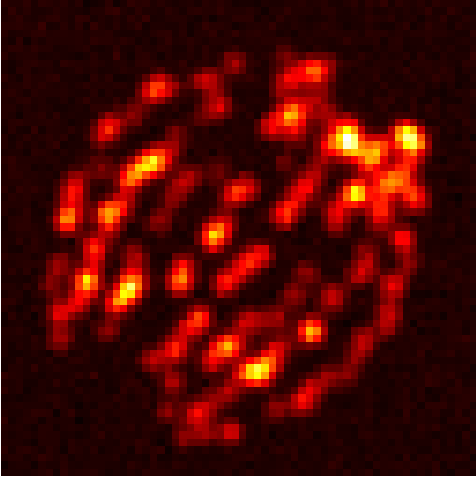
\includegraphics[width = 0.485\textwidth]{pictures/bundledTubesHighDensityFrameFarbig.png}}\hfill
\subfloat[Low spot density]{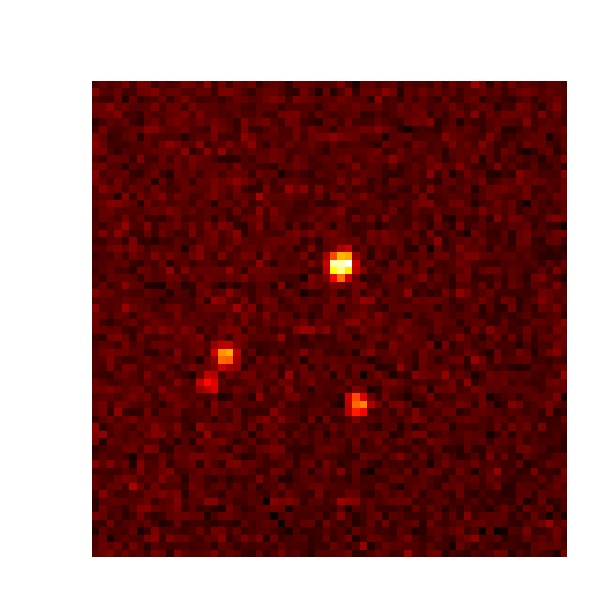
\includegraphics[width = 0.485\textwidth]{pictures/bundledTubesLowDensityFrameFarbig.png}}
	\caption{One frame from bundled tubes training data set}
	\label{bundledtubesHighowDensityFrame}	
\end{minipage}\hfill
\begin{minipage}[t]{0.33\textwidth}
\centering
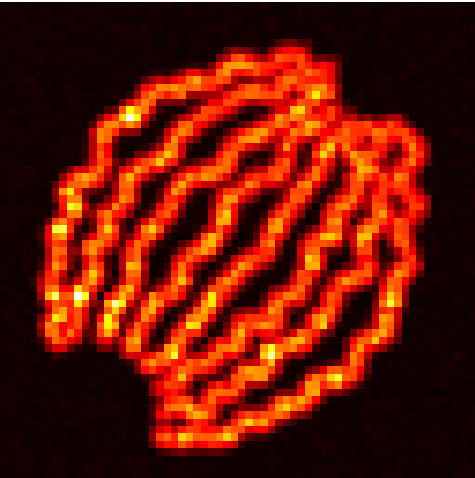
\includegraphics[width = 0.88\textwidth]{pictures/maximumProjectionBundledTubesLSFarbig.png}
	\caption{Maximum projection of bundled tubes data set}
	\label{pctMaximumProjBundledTubes}

\end{minipage}
\end{figure}
The original images very small, just 64 pixels in each dimension. Both sequences had spatial and temporal constant background. Picture \ref{pctMaximumProjBundledTubes} shows the maximum projection of the bundled tubes data set. The maximum projection is used to reduce the dimensionality of a data set. In this case for each pixel in $x$- and $y$-dimension, in the three dimensional dataset, the brightes value from all frames is taken. 


\subsection{Tubulin data sets}
The other training data sets models 7 microtubules, a structure that is a long filament up several micrometers long and a diameter of about 25 nanometers. The spot density lies somewhere between the high density and the low density of the bundled tubes data sets. This data sets show strong inhomogeneity in spatial dimensions and moderate inhomogeneity in temporal dimension, see figure \ref{tubulinVariableBg}. This is the reason why in the lower left corner of the maximum projection \ref{pctMaximumProjTubulin} a brighter area can be seen.

\begin{figure}
\subfloat[Tubulin2 frame 10]{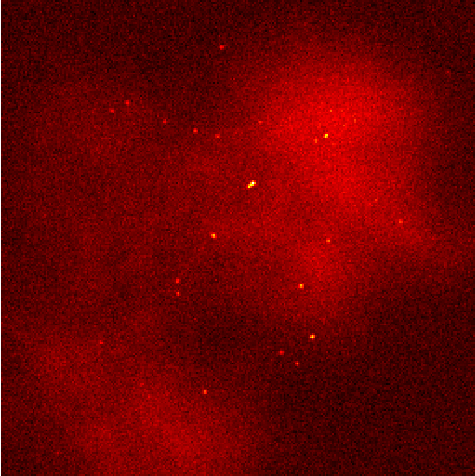
\includegraphics[width = 0.485\textwidth]{pictures/Tubulin2Frame10.png}}\hfill
\subfloat[Tubulin2 frame 1010]{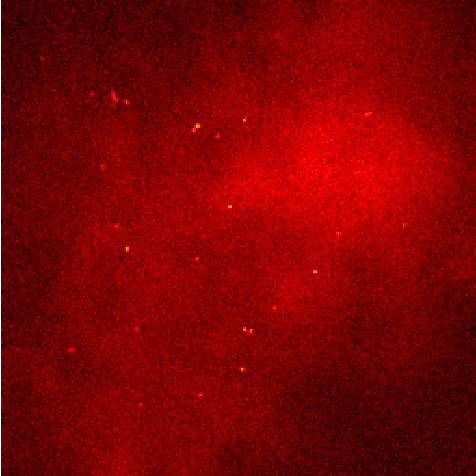
\includegraphics[width = 0.485\textwidth]{pictures/Tubulin2Frame1010.png}}
	\caption{This pictures show the variability of the background in the spatial and temporal dimensions}
	\label{tubulinVariableBg}	
\end{figure}

\begin{figure}
\centering
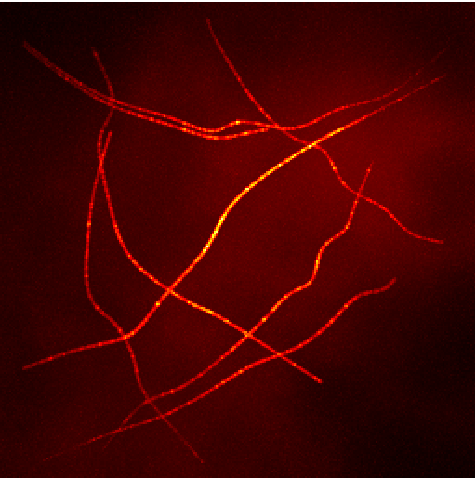
\includegraphics[width = 0.88\textwidth]{pictures/maximumProjectionTubulinFarbig.png}
	\caption{Maximum projection of tubulin data set}
	\label{pctMaximumProjTubulin}


\end{figure}

\section{Submissions}
\subsection{High precision}
\subsection{High score}
\subsection{Highest score via postprocessing}
\section{Results}
%\chapter{Data processing}
\section{the camera}
\subsection{dark current}

\section{the data}
The datasets for STORM microscopy that we recieve from our collaborators from
Bioquant are big datasets of several gigabyte in the Andor .sif format. Each
file conains a stack of pictures, normaly between 1000 and 10000, taken
consecutively.
In each picture there are beads and signals. Both result from very small 
fluorescent molecules attached to the structures that are investigated. The
light of this pointlike objects is dissorted to a gaussian shaped signal due to
the large magnification.
Beads are molecules that emit light at any time contrary to the other signal
which blinks that means it is visible in just one frame at an explicit location.
The beads are used as landmarks for later alignment of two or more different
color channels. The other spots are the structure that the biologist are
interested in. Each of the gaussian shaped signals should be recognized and the
center will be determined with subpixel accuracy and is stored in the end in a
list to be further processed by the colorcomposer application.

\section{Parameters and options}
\subsection{Necessary}

\section{Import and processing}
The STORM data has usually a size of around 3 gigabyte. There are even larger datasets possible, so that it is important to work on smaller parts of the data, instead putting the whole dataset into memory. This is done using chunks of user defined size. The data is processed chunkwise, there is parallelisation for the frames of each chunk. This is possible because the signals in each frame are considered to be independent from each other.  

\section{Workflow}
\subsection{Chose parameters}
At the begining the user has the option to set all important parameters, if no parameter is set the default ones are used and will give a good result because all crucial parameters are either determined from the data or set to reasonable values that work for every data set.
\subsection{Estimating camera gain and offset}
First of all it is checked whether there exists a file containing settings for gain and offset from an earlier run. If this is not the case new parameters are estimated based on the first part of the data, usually 200 frames are sufficiant.
The method described by \cite{skellam} is used to estimate the
gain factor. For this methode a Skellam distribution is used. 
Each dataset is three-dimensional where time is the third
dimension. Therefore mean $\mu$ and variance $\sigma^2$ can be calculated from
the data for each pixel individually
\begin{align}
	\mu(i,j) & = \frac{\Sigma_t(I_t(i,j)-I_{t+1}(i,j))}{n}\\
	\sigma^2 & = \frac{\Sigma_t(\mu-(I_t(i,j)-I_{t+1}(i,j)))^2}{n-1}
\end{align} 
To determine the gain factor the Skellam parameter are plotted over the mean
intensities. A straight line can be fitted and its slope is exactly the gain
factor.
\subsection{Recursevly adjusting gain and offset}
After the estimation of gain factor and offset, the transformation described in \ref{trafoPoiss} is applied.
\subsection{Estimating the width of the point spread function}
\subsection{Processing the data}
\subsubsection{Background estimation}
\subsubsection{Filter data}
\subsubsection{Find maxima}
\subsubsection{Quality control for detections}





\section{Background estimation}


\section{Mask for noise supression}
\section{Calibration measurement and plausibility}


\section{Accuracy of detection}
Unfortunately the position of the flourescent molecules can't be detected
perfectly. There are three main contribution to the error in detection.\\
First, there is the problem of finding the maximum in a noisy signal. Due to
noise the pixel next to the true maximum might get some intensity and be
therefore brighter.\\
Second, the choice of the gain factor and the offset might influence the
precision.\\
Third, the position is deteted by upscaling the pixel grid and interpolation.
After that the maximums position of the upscaled grid is taken as the resulting
position. This gives an error from roughly pixelwidth divided by square root of
two.
\subsection{error from noise}
Because there is no ground truth availible for micoscropy data, data must be
generated. This was done similar as described by \cite{simulated}.
\subsection{error from parameter estimation}

\section{Comparison with older version of the storm algorithm}
\section{Bleaching signal}

\section{Check for slope using calibration}
As described by \cite{meanVar} the true slope can be determined.

\section{New graphical user Interface}

%\chapter{Multicolor registration}
\section{Background}
In microscopy it is often desirable to label different structures in a cell with
different colors. To do so our collaborators use different fluoroscent molecules
that emit light at different and distinguishable wavelengths. Using different
filters it is possible to capture pictures just containing light emited from one
fluorophore. To get a mulit-channel picture the different channels must be
aligned. Because different flourophores emit different wavelengths, cromatic
aberration apears. This means that the light for the same spot but with
different wavelenghts is not mapped to the same spot in the image. To align the
different channels despite cromatic aberration, beads are used. Beads are
flourophores added to the probe, that emit light in all wavelengths the
different markers do and therefore are visible in all channels. The beads can be
used as landmarks, because their position in the original image is at the same
spot. The task is to find a transformation that maps corresponding beads on each
other.
\section{Features of the colercomposer application}

\section{Bead detection}
The input for the colorcomposer application is a text file created by the storm
algorithm that contains information about the position, intensity, symmetry,
framenumber and signal-to-noise ratio of each detection. The beads should
ideally be visible in most of the images, this means one must search for
detections that appear in almost every frame at the same position. Therefore it
is plausible to take every detection of the first 50 frames as initial
candidates for beads. After that candidates that are closer than a threshold are
merged to get a list of all location where beads might be. Given that list every
other detection is tested to belong to one of the bead candidates. If a
candidate gets too few members it is no longer considered to be a bead and
removed from the list.
\section{Align Beads}
After the beads for each channel are found the next task is to find the same
bead in each channel. It can happen that some beads occure in just one channel,
if this is the case there will be no corresponding bead in the other
channels.\\
To do so, the minimal number of beads, three to four, that are neccesary to
calculate the transformation are chosen randomly from the first channel. After that, based on
a probabilistic approach and a distance matrix containing information about the
distances between all beads of the two channels, three to four beads from the
second channel are chosen.\\
Using this pairs of beads linear transformation is found like described by
\cite{MAJoachim}. Using this transformation it is tested how many beads match in
total. It is assumed that the correct transformation will match other bead pairs
that were not chosen to calculate this transformation. After that the whole
procedure is done multiple times. In the end the best transformation is
chosen.\\
In principle shearing should also be allowed for this transformation, but tests
indicate that shearing does not occure. There is a problem if there are just
three beads in each channel, then every time a perfect transformation is found,
but with the constraint of forbidden shearing, the right solution can be
identified.

\section{Accuracy of Registration}

\section{Colocalisation}
\subsection{Global colocalisation}
\subsection{Local colocalisation}
\subsection{Validation of colocalisation approaches}
"Image set CBS001RGM-CBS010RGM from the Colocalization Benchmark Source
(www.colocalization-benchmark.com) was used to validate colocalization."

%\chapter{Work for the biologists}
\section{Selecting the best camera}


\section{little tool to investigate bleaching}


%\chapter{Futur work}
\section{3d Storm}

%%Ausblick schreiben!!!!!!!!~!!!
%\chapter{CCD camera}

\section{Image acquisition}
\subsection{Photon sources with shot noise}
The emission of photons is a random process that occures at unpredictible times. Therefore the number of photons passing through a plane is never constant but varies around some average value. The phenomena, that one can never determine exactly how many photons should hit the sensor chip of a CCD camera for example, is called shot noise. It playes a major role if the total number of photons is low, as from dark sources or with short exposure times of the camera.
\subsection{Quantum efficiency}
Quantum efficiency describes the fraction of photons that create a detectable electron in a sensor chip. The quantum efficiency is dependent of the wavelenght of the incoming photon. Photons with energies below the band gap can't produce a free electron that can be detected. The quantum efficiency has a maximum basically caused by two effects. The higher the photons energy the higher the kinetic energy of the freed electron, but it is absorbed earlier and can therefore recombinate with a electron hole more likely.
\subsection{Gain}
There are two different gain factors involved in the capturing process of a camera. First the electric signal for each pixel might be amplified. And there is also a gain factor that describes the proportionality between collected electrons and the digital number it is associated with.
\subsection{Readout noise}
The origin of readout noise is the amplifier. The aplification is never perfect, this means the exact number of electrons at the end of the amplification has some variation around the expected linearly increased value. There might also be some random signals of the electronics that add to the "true" signal. The readout noise is independent of the exposure time.
\subsection{Dark current noise}
Dark current noise is generated by the thermal movement of the atoms in the sensor chip. The movement of molecules and atoms is dependent of the temperature of the material, because of that dark current noise depends strongly on the temperature of the chip and can be reduced by cooling. Dark current noise generates electrons in the bins of each pixel even with closed shutter it is constantly increasing with time and follows Poisson statistics.
\subsection{Quantisation}
The signal must fit into the output color depth. It has to be rounded or truncated to fit in. This process introduces errors that can be seen as additional noise that is dependent on the intensity of the signal. High intensities are disturbed less relative to low intensies.

%\chapter{Appendix}


\listoffigures
\listoftables

\section{Additional tables of ISBI challenge results}

%\begin{table}[H]
\begin{center}
%\caption{Results for the main submission (with postprocessing)}
\begin{minipage}{\textwidth}
\captionof{table}{Results for the main submission for the high density data set (with postprocessing)}\label{reshd1}%
\begin{tabular}{lrrrr}
Dataset&Jaccard (in \%)&Precsision (in \%)& Recall (in \%) & RMSE (in nm)\\
HD1&40.44&100&41&40.13\\
HD2&30.84&100&31&63.18\\
HD3&12.55&100&13&61.8
\end{tabular} 
\end{minipage}
\end{center}
%\end{table}


%\begin{table}[H]
\begin{center}
\begin{minipage}{\textwidth}
\captionof{table}{Results for the high precission submission for the high density data set}\label{reshd2}
\begin{tabular}{lrrrr}
Dataset&Jaccard (in \%)&Precsision (in \%)& Recall (in \%) & RMSE (in nm)\\
HD1&37.62&100&38&40.23\\
HD2&28.37&100&28&60.70\\
HD3&12.66&100&13&62.58
\end{tabular}
\end{minipage}
\end{center}
%\end{table}

\begin{center}
\begin{minipage}{\textwidth}
\captionof{table}{Results for the high score submission for the high density data set (without postprocessing)}\label{reshd3}
\begin{tabular}{lrrrr}
Dataset&Jaccard (in \%)&Precsision (in \%)& Recall (in \%) & RMSE (in nm)\\
HD1&37.96&100&38&40.22\\
HD2&29.73&94&30&63.33\\
HD3&13.00&99&13&63.95
\end{tabular}
\end{minipage}
\end{center}


\begin{center}
\begin{minipage}{\textwidth}
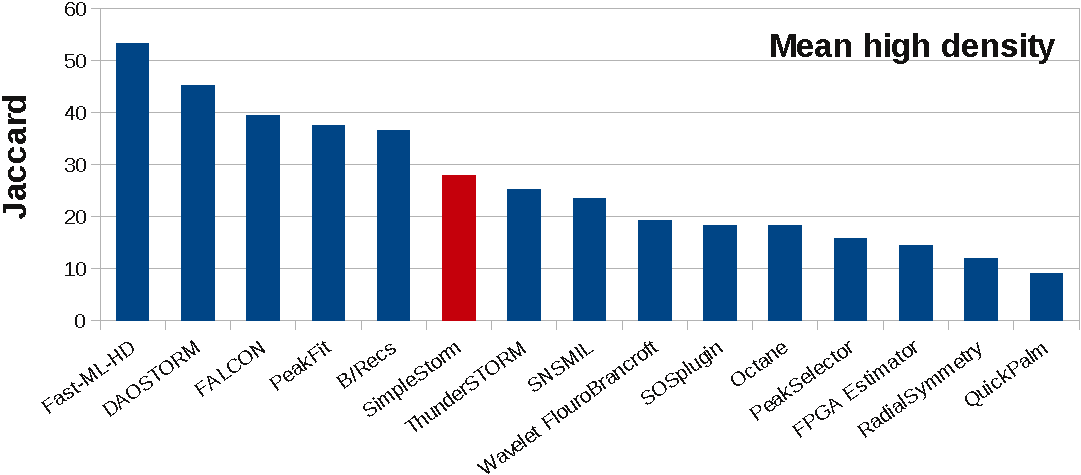
\includegraphics[width = 0.88\textwidth]{pictures/diagrammsChallenge/MeanHighDensityJaccardCropped.pdf}
	\captionof{figure}{Results for high density data sets. The Jaccard indices are averaged over all three data sets. For this score higher is better.}
	\label{meanJaccardHighDensity}
	\end{minipage}
\end{center}

\begin{center}
\begin{minipage}{\textwidth}
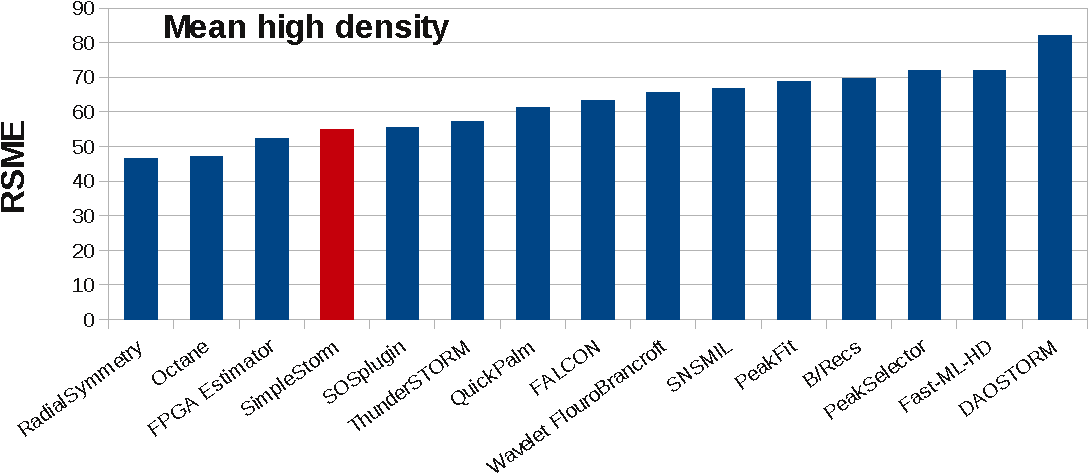
\includegraphics[width = 0.88\textwidth]{pictures/diagrammsChallenge/MeanHighDensityRSMECropped.pdf}
	\captionof{figure}{Results for high density data sets. Averaged RSME scores over all three datasets. For this score lower is better.}
	\label{meanRSMEHighDensity}
	\end{minipage}
\end{center}



\begin{center}
\begin{minipage}{\textwidth}
\captionof{table}{Results for the main submission for low density data sets(with postprocessing)}
\begin{tabular}{lrrrr}
Dataset&Jaccard (in \%)&Precsision (in \%)& Recall (in \%) & RMSE (in nm)\\
LS1&86.12&100&86&26.32\\
LS2&69.64&97&71&37.43\\
LS3&47.48&99&48&54.2
\end{tabular}\label{resls1}
\end{minipage}
\end{center}


\begin{center}
\begin{minipage}{\textwidth}
\captionof{table}{Results for the high precission submission for low density data sets}\label{resls2}
\begin{tabular}{lrrrr}
Dataset&Jaccard (in \%)&Precsision (in \%)& Recall (in \%) & RMSE (in nm)\\
LS1&83.39&100&83&27.91\\
LS2&63.21&100&63&39.57\\
LS3&40.82&100&41&49.55
\end{tabular}
\end{minipage}
\end{center}

\begin{center}
\begin{minipage}{\textwidth}
\captionof{table}{Results for the high score submission for low density data sets (without postprocessing)}\label{resls3}
\begin{tabular}{lrrrr}
Dataset&Jaccard (in \%)&Precsision (in \%)& Recall (in \%) & RMSE (in nm)\\
LS1&87.23&99&88&28.10\\
LS2&65.95&89&72&44.60\\
LS3&40.82&96&48&54.40
\end{tabular}
\end{minipage}
\end{center}



\begin{center}
\begin{minipage}{\textwidth}
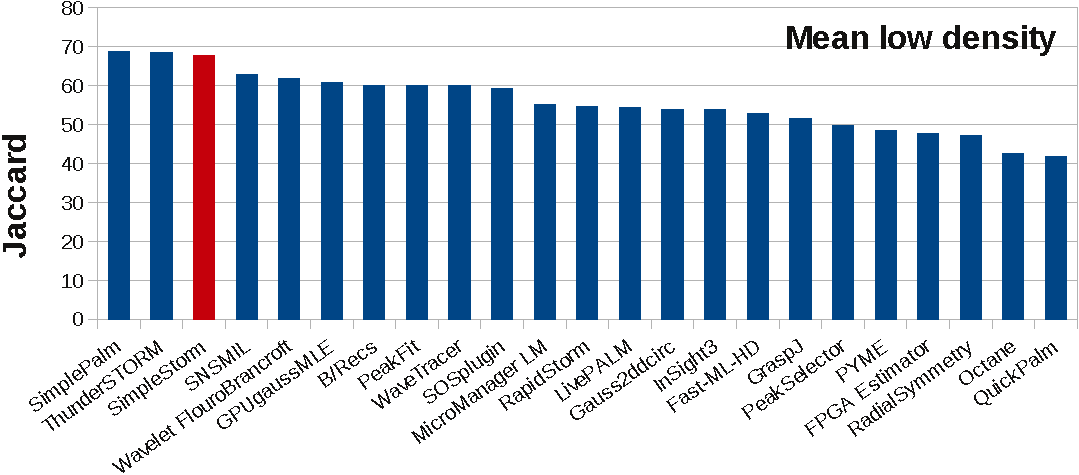
\includegraphics[width = 0.88\textwidth]{pictures/diagrammsChallenge/MeanLowDensityJaccardCropped.pdf}
	\captionof{figure}{Results for low density data sets. The Jaccard indices are averaged over all three data sets. For this score higher is better.}
	\label{meanJaccardLowDensity}
\end{minipage}
\end{center}

\begin{center}
\begin{minipage}{\textwidth}
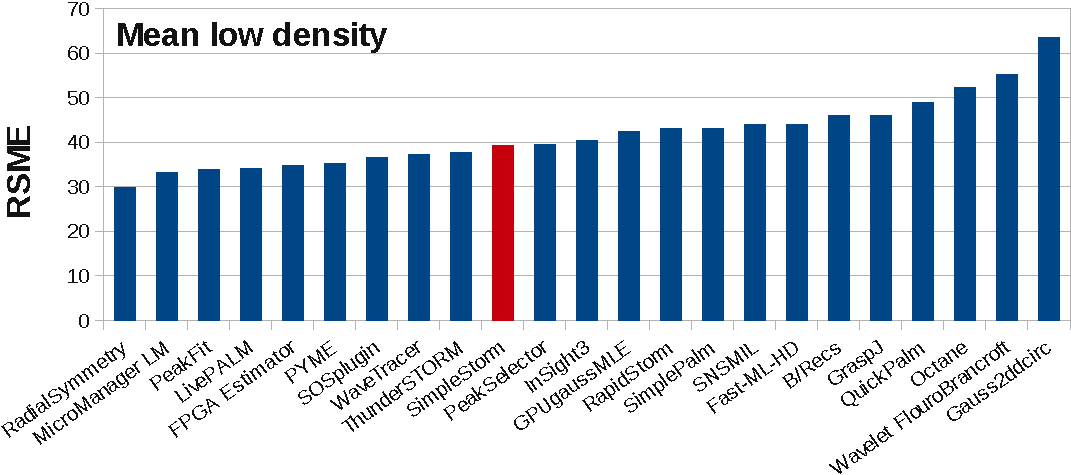
\includegraphics[width = 0.88\textwidth]{pictures/diagrammsChallenge/MeanLowDensityRSMECropped.pdf}
	\captionof{figure}{Results for low density data sets. Averaged RSME scores over all three datasets. For this score lower is better.}
	\label{meanRSMELowDensity}
\end{minipage}
\end{center}

\begin{center}
\begin{minipage}{\textwidth}
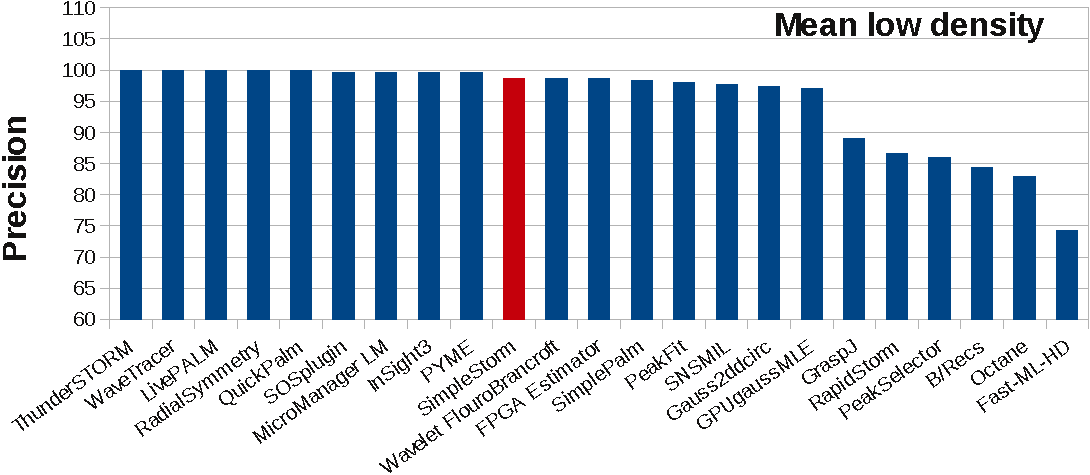
\includegraphics[width = 0.88\textwidth]{pictures/diagrammsChallenge/MeanLowDensityPrecisionCropped.pdf}
	\captionof{figure}{Results for low density data sets. Averaged Precision over all three datasets. For this score higher is better. The y axis is broken to show the differences better.}
	\label{meanPrecisionLowDensity}
\end{minipage}
\end{center}

\begin{center}
\begin{minipage}{\textwidth}
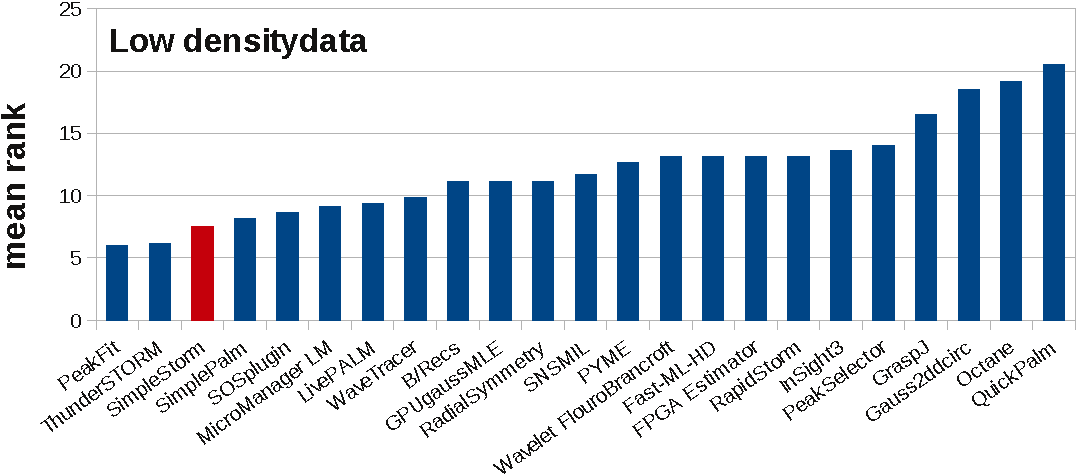
\includegraphics[width = 0.88\textwidth]{pictures/diagrammsChallenge/MeanRankLowDensityCropped.pdf}
	\captionof{figure}{Averaged rank over Jaccard index and RSME score for all low density data sets. Lower ranks are better.}
	\label{meanRankLow}
\end{minipage}
\end{center}

\begin{center}
\begin{minipage}{\textwidth}
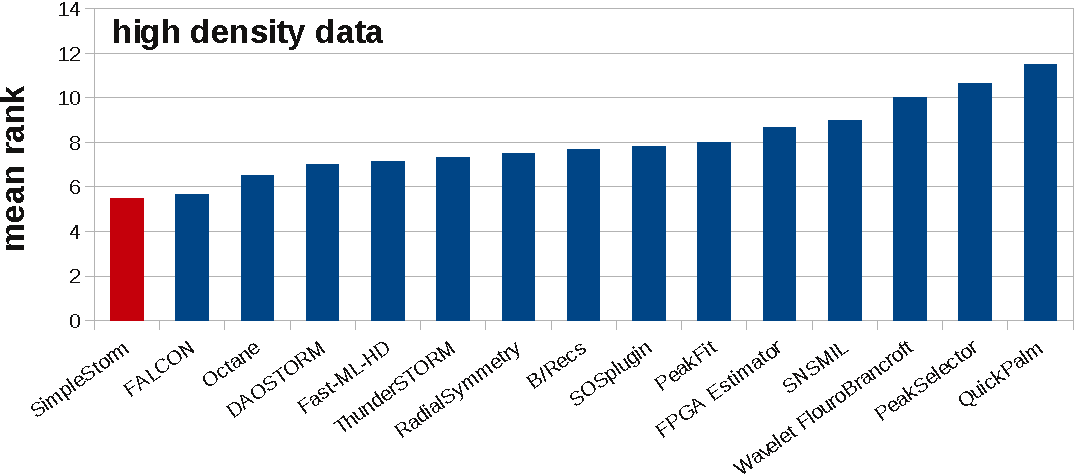
\includegraphics[width = 0.88\textwidth]{pictures/diagrammsChallenge/MeanRankHighDensityCropped.pdf}
	\captionof{figure}{Averaged rank over Jaccard index and RSME score for all high density data sets. Lower ranks are better}
	\label{meanRankHigh}
	\end{minipage}
\end{center}
%\begin{thebibliography}{9}
\bibitem{skellam} Hwang, Youngbae; Hun-Sik, Kim; Kweon, In So
\textit{Difference-Based Image Noise Modeling Using Skellam Distribution}, IEEE
Transactions on Pattern Analysis and Machine Intelligence \textbf{34}, 7 1329
(2012) 
\bibitem{teflon} Touloukian,Y.
S.
; Kirby,R.
K.
; Taylor,E.
R.
; Lee,T. Y. R.,
\textit{Thermophysical Properties of Matter - the TPRC Data Series.} 
\textbf{13} Thermal Expansion - Nonmetallic Solids,New York : IFI/Plenum, (1977)
\bibitem{characterization} Gang Zou;    Gronqvist, H.;    Starski, J.P.;   
Johan Liu;   \textit{Characterization of liquid crystal polymer for high
frequency system-in-a-package applications}; Advanced Packaging, IEEE
Trans.  \textbf{25}, 4 503 (2002)
\bibitem{microwave} 
Jacob, M.V.;   Mazierska, J.;   Leong, K.;   Krupka, J.;   \textit{Microwave
properties of low-loss polymers at cryogenic temperatures} Microwave Theory and
Techniques, IEEE Trans. \textbf{50},2 474 (2002) 
\bibitem{rogers1} http://www.hofmannlp.de/pub/rt5880.pdf
\bibitem{rogers2}
http://www.rogerscorp.com/documents/730/acm/ULTRALAM-3000-LCP-laminate-data-sheet-ULTRALAM-3850.aspx
\bibitem{julia} J. Bach, \textit{Mikrowellenspektroskopie mit
Streifenleitungen}, Diplom Arbeit, Universit�t Stuttgart (2009) 
\bibitem{marc} M. Scheffler, \textit{Broadband Microwave Spectroscopy on
Correlated Electrons}, PhD thesis, Universit�t Stuttgart (2004)

\end{thebibliography}
\bibliographystyle{te}

\bibliography{research}

\end{document}
